\documentclass{article}
\usepackage[T1]{fontenc}
\usepackage[utf8]{inputenc}
\usepackage[paperwidth=33.53cm,paperheight=22.86cm,margin=0cm]{geometry}
\usepackage{lmodern}
\usepackage{xcolor}
\usepackage{tikz}
\usetikzlibrary{arrows.meta,calc}

\pagestyle{empty}

% 6x9 trade trim with an approximate 1.20in spine for the current 534-page book.
% Update \SpineW to the final printer's exact specification before production.
\def\TrimW{15.24}
\def\TrimH{22.86}
\def\SpineW{3.05}
\def\FrontX{18.29}

\definecolor{coverBgTop}{HTML}{08121B}
\definecolor{coverBgBottom}{HTML}{11283A}
\definecolor{coverGrid}{HTML}{1D4255}
\definecolor{coverCard}{HTML}{F5F2E8}
\definecolor{coverInk}{HTML}{0A1B28}
\definecolor{coverSky}{HTML}{8FD7FF}
\definecolor{coverTeal}{HTML}{48D1C2}
\definecolor{coverAmber}{HTML}{F3B34C}
\definecolor{coverCoral}{HTML}{E57D63}
\definecolor{coverSlate}{HTML}{9DB1BE}
\definecolor{coverRule}{HTML}{365F73}
\definecolor{coverTitle}{HTML}{F6F1E6}
\definecolor{coverAuthor}{HTML}{B6C3CC}
\definecolor{coverBackPanel}{HTML}{0E1C2A}
\definecolor{coverBackCard}{HTML}{F3EEDF}

\begin{document}
\noindent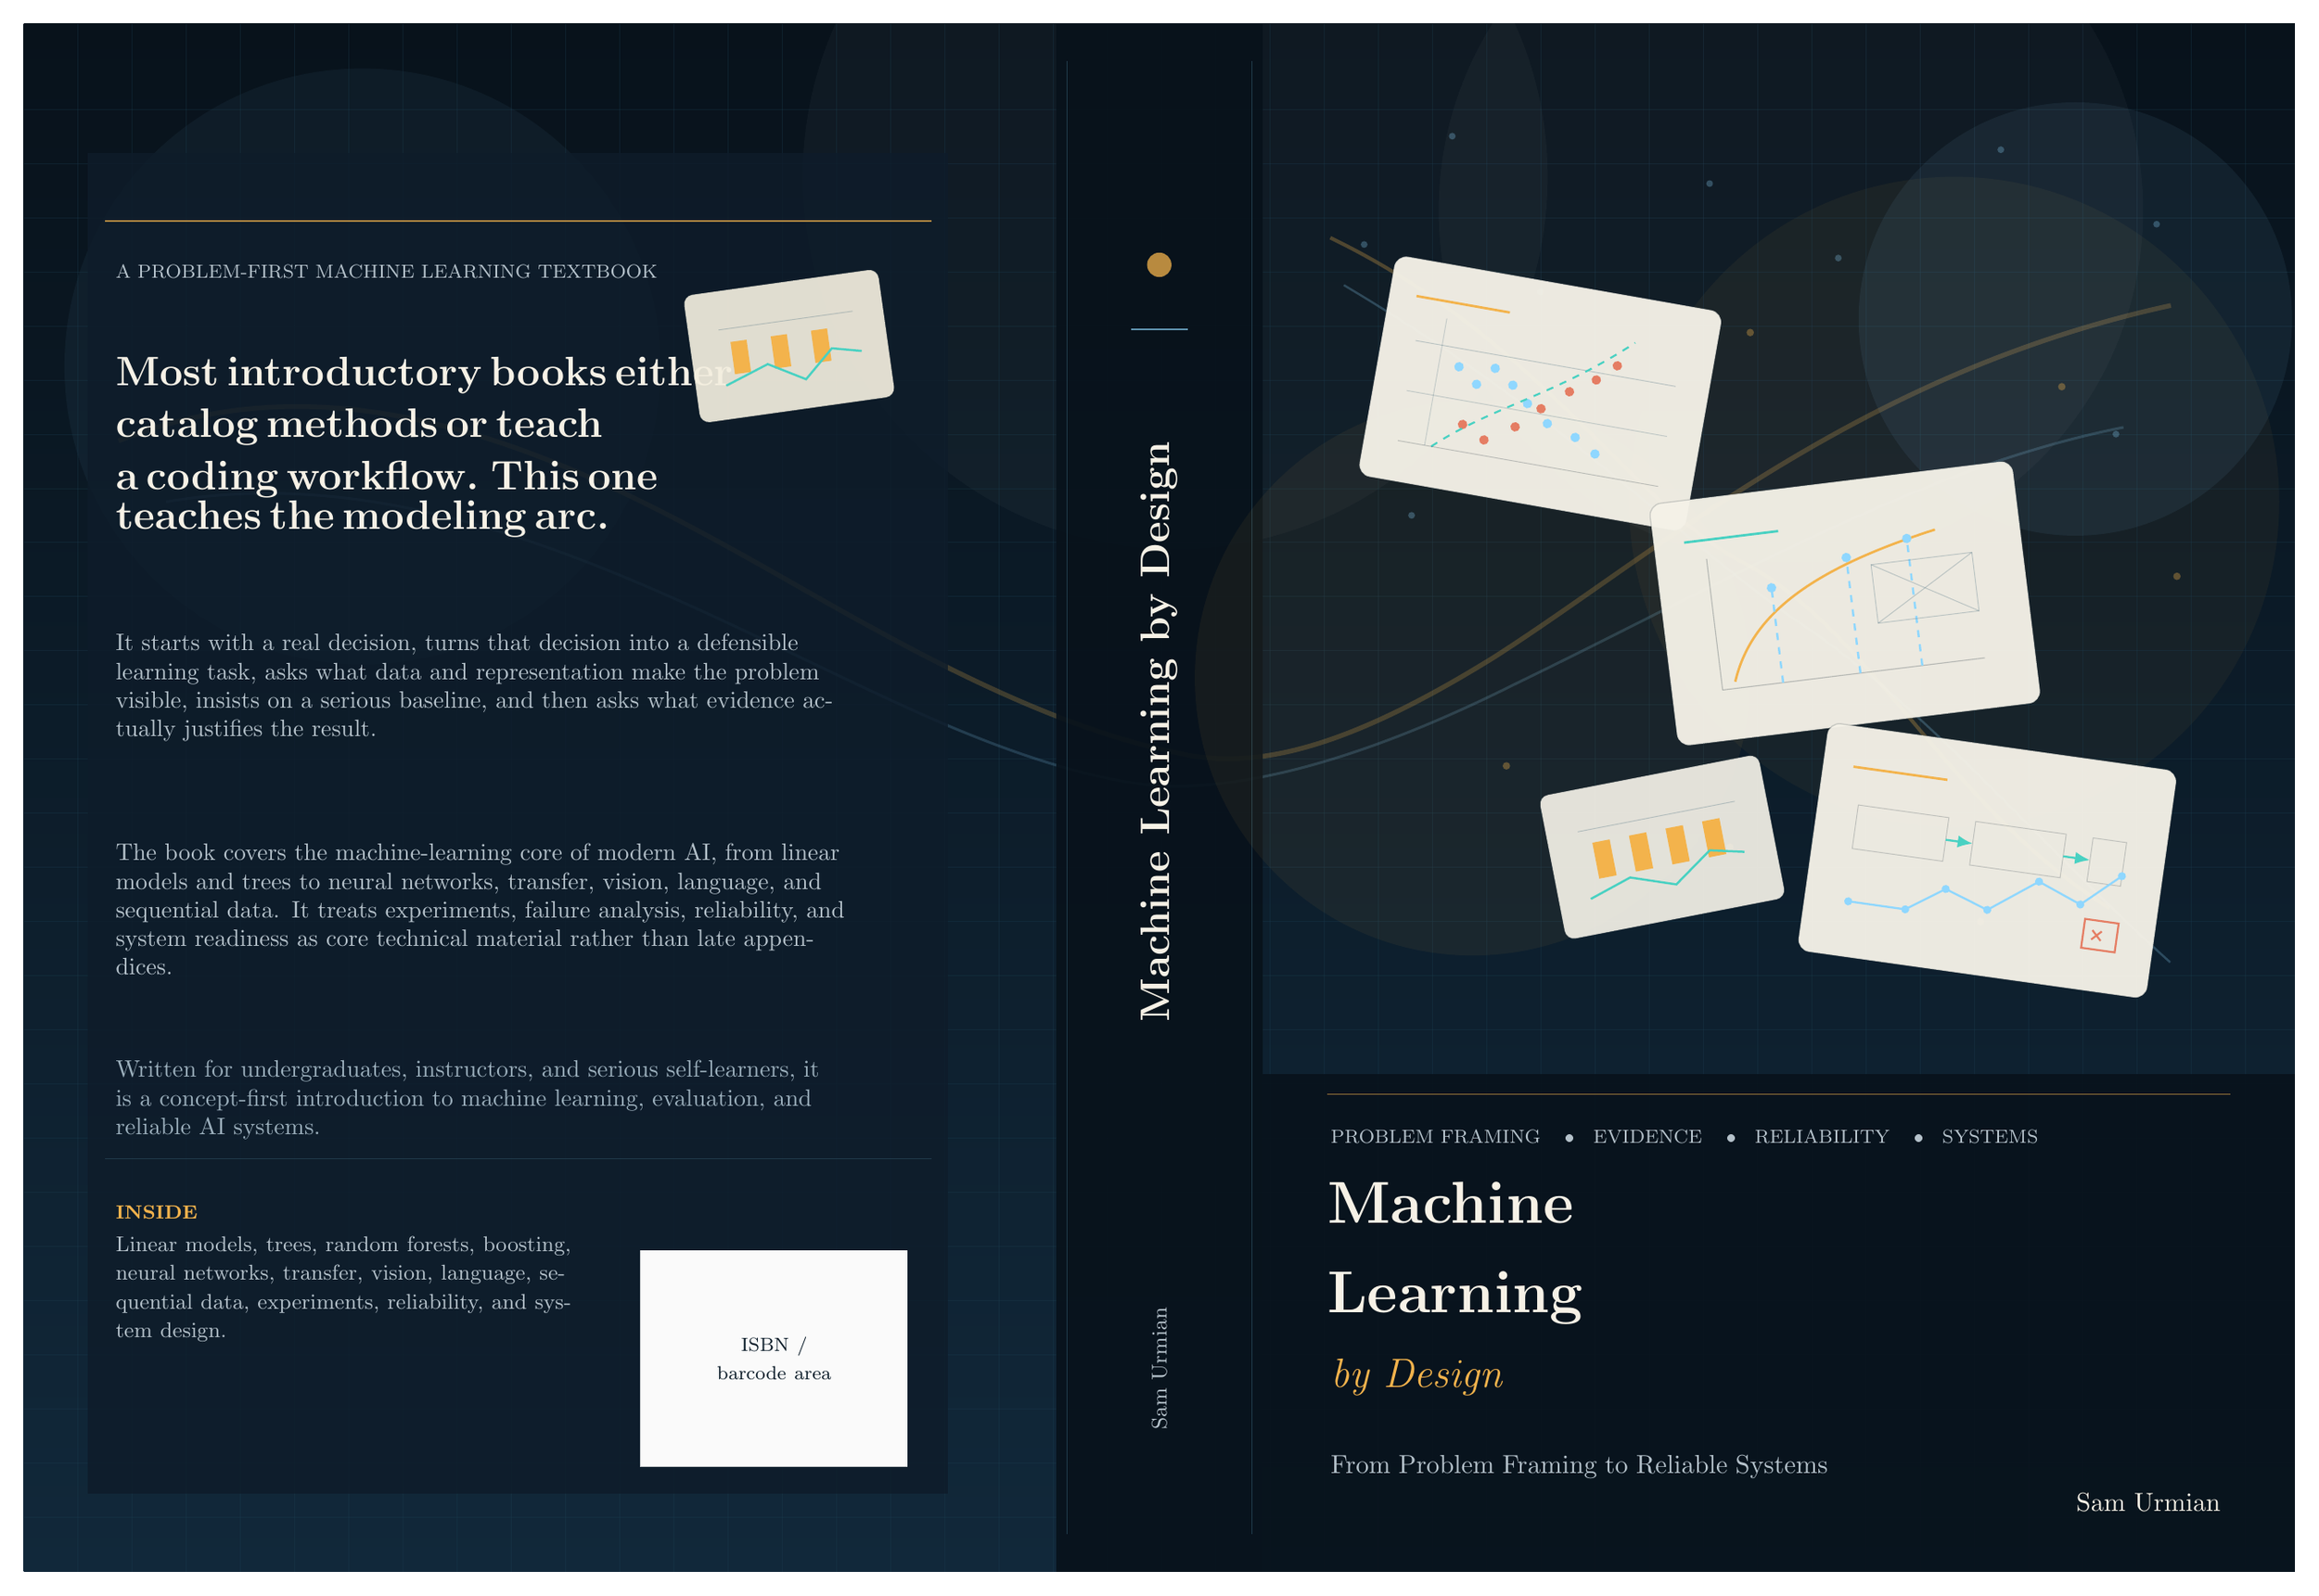
\begin{tikzpicture}[x=1cm,y=1cm]
  \useasboundingbox (0,0) rectangle ({2*\TrimW+\SpineW},\TrimH);

  % Wrap background
  \shade[top color=coverBgTop,bottom color=coverBgBottom] (0,0) rectangle ({2*\TrimW+\SpineW},\TrimH);
  \fill[coverSky,opacity=0.05] (5.0,17.8) circle (4.4cm);
  \fill[coverAmber,opacity=0.05] (28.5,15.8) circle (4.8cm);
  \fill[white,opacity=0.03] (17.0,20.6) circle (5.5cm);

  \foreach \gx in {0.8,1.6,...,33.2}{
    \draw[coverGrid,opacity=0.30,line width=0.22pt] (\gx,0) -- (\gx,\TrimH);}
  \foreach \gy in {0.8,1.6,...,22.4}{
    \draw[coverGrid,opacity=0.30,line width=0.22pt] (0,\gy) -- ({2*\TrimW+\SpineW},\gy);}

  % Continuous gesture across the wrap
  \draw[coverAmber,opacity=0.22,line width=2.0pt]
    (1.4,16.7) .. controls (5.6,18.4) and (9.8,15.4) .. (12.6,13.9)
    .. controls (14.6,12.8) and (16.0,12.3) .. (17.0,12.1)
    .. controls (18.2,11.8) and (19.6,12.2) .. (21.7,13.5)
    .. controls (24.2,15.1) and (27.1,17.7) .. (31.7,18.7);
  \draw[coverSky,opacity=0.18,line width=1.1pt]
    (2.1,15.8) .. controls (6.2,16.5) and (10.0,14.1) .. (13.4,12.6)
    .. controls (15.0,11.9) and (16.2,11.6) .. (17.0,11.6)
    .. controls (18.0,11.6) and (19.6,11.9) .. (22.0,13.1)
    .. controls (25.3,14.7) and (28.0,16.3) .. (31.0,16.9);

  % Back panel copy area
  \fill[coverBackPanel,opacity=0.82] (0.95,1.15) rectangle (13.65,20.95);
  \draw[coverAmber,opacity=0.70,line width=0.65pt] (1.20,19.95) -- (13.40,19.95);
  \draw[coverRule,opacity=0.45,line width=0.45pt] (1.20,6.10) -- (13.40,6.10);

  \node[anchor=west,inner sep=0pt] at (1.35,19.20)
    {\fontsize{8.5}{10}\selectfont\rmfamily\color{coverAuthor}A PROBLEM-FIRST MACHINE LEARNING TEXTBOOK};

  \node[anchor=north west,align=left,text width=11.0cm,inner sep=0pt] at (1.35,17.95)
    {\raggedright\fontsize{19}{22}\selectfont\bfseries\rmfamily\color{coverTitle}Most introductory books either\\catalog methods or teach\\a coding workflow. This one\\teaches the modeling arc.};

  \node[anchor=north west,align=left,text width=10.9cm,inner sep=0pt] at (1.35,13.85)
    {\raggedright\fontsize{10.2}{13.3}\selectfont\rmfamily\color{coverAuthor}It starts with a real decision, turns that decision into a defensible learning task, asks what data and representation make the problem visible, insists on a serious baseline, and then asks what evidence actually justifies the result.};

  \node[anchor=north west,align=left,text width=10.9cm,inner sep=0pt] at (1.35,10.75)
    {\raggedright\fontsize{10.2}{13.3}\selectfont\rmfamily\color{coverAuthor}The book covers the machine-learning core of modern AI, from linear models and trees to neural networks, transfer, vision, language, and sequential data. It treats experiments, failure analysis, reliability, and system readiness as core technical material rather than late appendices.};

  \node[anchor=north west,align=left,text width=10.9cm,inner sep=0pt] at (1.35,7.55)
    {\raggedright\fontsize{9.7}{12.8}\selectfont\rmfamily\color{coverSlate}Written for undergraduates, instructors, and serious self-learners, it is a concept-first introduction to machine learning, evaluation, and reliable AI systems.};

  \node[anchor=west,inner sep=0pt] at (1.35,5.30)
    {\fontsize{8.2}{10}\selectfont\bfseries\rmfamily\color{coverAmber}INSIDE};
  \node[anchor=north west,align=left,text width=7.1cm,inner sep=0pt] at (1.35,4.95)
    {\raggedright\fontsize{9.2}{12}\selectfont\rmfamily\color{coverAuthor}Linear models, trees, random forests, boosting, neural networks, transfer, vision, language, sequential data, experiments, reliability, and system design.};

  % Barcode placeholder
  \fill[white,opacity=0.98] (9.10,1.55) rectangle (13.05,4.75);
  \draw[coverInk,opacity=0.22,line width=0.45pt] (9.10,1.55) rectangle (13.05,4.75);
  \node[anchor=center,align=center,text width=3.2cm] at (11.08,3.15)
    {\fontsize{8}{10}\selectfont\rmfamily\color{coverInk}ISBN /\\barcode area};

  % Small back motif
  \begin{scope}[shift={(11.3,18.1)},rotate=8]
    \fill[coverBackCard,opacity=0.92,rounded corners=0.14cm] (-1.45,-0.95) rectangle (1.45,0.95);
    \draw[coverInk,opacity=0.16,line width=0.35pt,rounded corners=0.14cm] (-1.45,-0.95) rectangle (1.45,0.95);
    \draw[coverRule,opacity=0.28,line width=0.35pt] (-1.0,0.38) -- (1.0,0.38);
    \foreach \x in {-0.85,-0.25,0.35}{
      \fill[coverAmber] (\x,-0.30) rectangle ++(0.24,0.48);}
    \draw[coverTeal,line width=0.9pt] (-1.0,-0.45) -- (-0.35,-0.22) -- (0.18,-0.52) -- (0.62,-0.12) -- (1.05,-0.22);
  \end{scope}

  % Spine
  \fill[coverBgTop,opacity=0.92] (\TrimW,0) rectangle ({\TrimW+\SpineW},\TrimH);
  \draw[coverRule,opacity=0.55,line width=0.45pt] (\TrimW+0.16,0.55) -- (\TrimW+0.16,22.31);
  \draw[coverRule,opacity=0.55,line width=0.45pt] ({\TrimW+\SpineW-0.16},0.55) -- ({\TrimW+\SpineW-0.16},22.31);
  \node[rotate=90,anchor=center] at ({\TrimW+0.5*\SpineW},12.4)
    {\fontsize{16}{18}\selectfont\bfseries\rmfamily\color{coverTitle}Machine Learning by Design};
  \node[rotate=90,anchor=center] at ({\TrimW+0.5*\SpineW},3.0)
    {\fontsize{9.2}{11}\selectfont\rmfamily\color{coverAuthor}Sam Urmian};
  \fill[coverAmber,opacity=0.75] ({\TrimW+0.5*\SpineW},19.3) circle (0.18cm);
  \draw[coverSky,opacity=0.65,line width=0.7pt] ({\TrimW+0.5*\SpineW-0.42},18.35) -- ({\TrimW+0.5*\SpineW+0.42},18.35);

  % Front cover art
  \begin{scope}[shift={(\FrontX,0)}]
    \fill[coverSky,opacity=0.07] (12.0,18.5) circle (3.2cm);
    \fill[coverAmber,opacity=0.06] (3.1,13.2) circle (4.1cm);
    \fill[white,opacity=0.03] (7.8,20.1) circle (5.2cm);

    \foreach \p in {(1.5,19.6),(2.8,21.2),(4.1,18.9),(6.6,20.5),(8.5,19.4),(10.9,21.0),(13.2,19.9),(12.6,16.8),(2.2,15.6)}{
      \fill[coverSky,opacity=0.28] \p circle (0.05cm);}
    \foreach \p in {(5.1,17.7),(7.2,18.3),(11.8,17.5),(13.5,14.7),(3.6,11.9),(6.9,10.7),(10.6,9.6)}{
      \fill[coverAmber,opacity=0.34] \p circle (0.055cm);}

    \draw[coverAmber,opacity=0.28,line width=1.5pt] (1.0,19.7) .. controls (4.1,18.2) and (5.4,15.8) .. (7.1,14.9)
      .. controls (9.0,13.9) and (10.1,11.3) .. (12.5,9.8);
    \draw[coverSky,opacity=0.24,line width=0.9pt] (1.2,19.0) .. controls (4.4,17.1) and (6.1,15.3) .. (7.8,14.1)
      .. controls (9.8,12.8) and (11.5,10.7) .. (13.4,9.0);

    \begin{scope}[shift={(4.1,17.4)},rotate=-10]
      \fill[coverCard,opacity=0.96,rounded corners=0.18cm] (-2.45,-1.65) rectangle (2.45,1.65);
      \draw[coverInk,opacity=0.18,line width=0.45pt,rounded corners=0.18cm] (-2.45,-1.65) rectangle (2.45,1.65);
      \draw[coverAmber,line width=1.0pt] (-2.05,1.10) -- (-0.65,1.10);
      \draw[coverRule,opacity=0.28,line width=0.35pt] (-1.95,0.45) -- (1.95,0.45);
      \draw[coverRule,opacity=0.24,line width=0.35pt] (-1.95,-0.30) -- (1.95,-0.30);
      \draw[coverRule,opacity=0.22,line width=0.35pt] (-1.55,-1.05) -- (-1.55,0.85);
      \foreach \p in {(-1.25,0.18),(-0.95,-0.03),(-0.72,0.25),(-0.42,0.05),(-0.16,-0.18),(0.18,-0.42),(0.62,-0.55),(0.95,-0.74)}{
        \fill[coverSky] \p circle (0.07cm);}
      \foreach \p in {(-1.05,-0.65),(-0.70,-0.82),(-0.28,-0.55),(0.05,-0.22),(0.42,0.10),(0.78,0.34),(1.05,0.60)}{
        \fill[coverCoral] \p circle (0.07cm);}
      \draw[coverTeal,dashed,line width=0.8pt] (-1.45,-1.05) .. controls (-0.65,-0.30) and (0.18,-0.02) .. (1.25,0.98);
      \draw[coverInk,opacity=0.22,line width=0.35pt] (-1.95,-1.05) -- (1.95,-1.05);
    \end{scope}

    \begin{scope}[shift={(8.6,14.3)},rotate=7]
      \fill[coverCard,opacity=0.96,rounded corners=0.18cm] (-2.70,-1.80) rectangle (2.70,1.80);
      \draw[coverInk,opacity=0.18,line width=0.45pt,rounded corners=0.18cm] (-2.70,-1.80) rectangle (2.70,1.80);
      \draw[coverTeal,line width=1.0pt] (-2.25,1.18) -- (-0.85,1.18);
      \draw[coverInk,opacity=0.24,line width=0.40pt] (-1.95,-1.05) -- (-1.95,0.90);
      \draw[coverInk,opacity=0.24,line width=0.40pt] (-1.95,-1.05) -- (1.95,-1.05);
      \draw[coverAmber,line width=1.0pt] (-1.75,-0.95) .. controls (-1.40,0.00) and (-0.45,0.56) .. (1.45,0.92);
      \draw[coverSky,line width=0.9pt,dashed] (-1.05,-1.05) -- (-1.05,0.36);
      \draw[coverSky,line width=0.9pt,dashed] (0.10,-1.05) -- (0.10,0.67);
      \draw[coverSky,line width=0.9pt,dashed] (1.02,-1.05) -- (1.02,0.84);
      \foreach \x/\y in {-1.05/0.36,0.10/0.67,1.02/0.84}{
        \fill[coverSky] (\x,\y) circle (0.07cm);}
      \draw[coverRule,opacity=0.28,line width=0.35pt] (0.45,-0.35) rectangle (1.95,0.52);
      \draw[coverRule,opacity=0.28,line width=0.35pt] (0.45,-0.35) -- (1.95,0.52);
      \draw[coverRule,opacity=0.28,line width=0.35pt] (0.45,0.52) -- (1.95,-0.35);
    \end{scope}

    \begin{scope}[shift={(10.7,10.5)},rotate=-8]
      \fill[coverCard,opacity=0.96,rounded corners=0.18cm] (-2.60,-1.70) rectangle (2.60,1.70);
      \draw[coverInk,opacity=0.18,line width=0.45pt,rounded corners=0.18cm] (-2.60,-1.70) rectangle (2.60,1.70);
      \draw[coverAmber,line width=1.0pt] (-2.15,1.10) -- (-0.75,1.10);
      \draw[coverInk,opacity=0.20,line width=0.35pt] (-2.00,0.55) rectangle (-0.65,-0.10);
      \draw[coverInk,opacity=0.20,line width=0.35pt] (-0.25,0.55) rectangle (1.10,-0.10);
      \draw[coverInk,opacity=0.20,line width=0.35pt] (1.50,0.55) rectangle (2.00,-0.10);
      \draw[coverTeal,line width=0.85pt,-{Latex[length=2.2mm,width=1.8mm]}] (-0.65,0.22) -- (-0.25,0.22);
      \draw[coverTeal,line width=0.85pt,-{Latex[length=2.2mm,width=1.8mm]}] (1.10,0.22) -- (1.50,0.22);
      \draw[coverSky,line width=0.85pt] (-1.95,-0.88) -- (-1.10,-0.88) -- (-0.55,-0.50) -- (0.10,-0.72) -- (0.80,-0.20) -- (1.45,-0.45) -- (2.00,0.05);
      \foreach \x/\y in {-1.95/-0.88,-1.10/-0.88,-0.55/-0.50,0.10/-0.72,0.80/-0.20,1.45/-0.45,2.00/0.05}{
        \fill[coverSky] (\x,\y) circle (0.06cm);}
      \draw[coverCoral,line width=0.80pt] (1.55,-1.08) rectangle (2.05,-0.65);
      \draw[coverCoral,line width=0.80pt] (1.68,-0.94) -- (1.82,-0.80);
      \draw[coverCoral,line width=0.80pt] (1.68,-0.80) -- (1.82,-0.94);
    \end{scope}

    \begin{scope}[shift={(5.9,10.7)},rotate=11]
      \fill[coverCard,opacity=0.92,rounded corners=0.14cm] (-1.65,-1.08) rectangle (1.65,1.08);
      \draw[coverInk,opacity=0.16,line width=0.40pt,rounded corners=0.14cm] (-1.65,-1.08) rectangle (1.65,1.08);
      \draw[coverRule,opacity=0.28,line width=0.35pt] (-1.18,0.46) -- (1.18,0.46);
      \foreach \x in {-1.00,-0.45,0.10,0.65}{
        \fill[coverAmber] (\x,-0.28) rectangle ++(0.26,0.54);}
      \draw[coverTeal,line width=0.9pt] (-1.18,-0.55) -- (-0.55,-0.35) -- (0.10,-0.58) -- (0.68,-0.18) -- (1.18,-0.30);
    \end{scope}

    \fill[coverBgTop,opacity=0.90] (0,0) rectangle (\TrimW,7.35);
    \draw[coverAmber,opacity=0.60,line width=0.65pt] (0.95,7.05) -- (14.29,7.05);
    \node[anchor=west,inner sep=0pt] at (1.00,6.42)
      {\fontsize{8.5}{10}\selectfont\rmfamily\color{coverAuthor}PROBLEM FRAMING \hspace{0.55em} \textbullet \hspace{0.55em} EVIDENCE \hspace{0.55em} \textbullet \hspace{0.55em} RELIABILITY \hspace{0.55em} \textbullet \hspace{0.55em} SYSTEMS};
    \node[anchor=base west,inner sep=0pt] at (0.95,5.15)
      {\fontsize{33}{37}\selectfont\bfseries\rmfamily\color{coverTitle}Machine};
    \node[anchor=base west,inner sep=0pt] at (0.95,3.82)
      {\fontsize{33}{37}\selectfont\bfseries\rmfamily\color{coverTitle}Learning};
    \node[anchor=base west,inner sep=0pt] at (1.00,2.72)
      {\fontsize{18}{22}\selectfont\itshape\rmfamily\color{coverAmber}by Design};
    \node[anchor=west,align=left,inner sep=0pt,text width=8.9cm] at (1.00,1.55)
      {\fontsize{10.5}{13}\selectfont\rmfamily\color{coverAuthor}From Problem Framing to Reliable Systems};
    \node[anchor=east,inner sep=0pt] at (14.15,1.02)
      {\fontsize{11}{13}\selectfont\rmfamily\color{coverTitle}Sam Urmian};
  \end{scope}
\end{tikzpicture}
\end{document}
